%!TEX root = ../MasterThesis.tex

\section{Concept of System}
\label{sec:system_concept}

Based on the explanations in Chapter~\ref{cha:context_analysis}, and especially the scope definition for this Master thesis in Section~\ref{sec:scope_thesis}, the collaborative system for investigating E-commerce fraud incidents have to answer the central question:\@

\begin{quotation}
    \textit{Is this really a fraudulent E-commerce transaction?}
\end{quotation}

The relevant stakeholders, that need to be involved in the investigation process, are:\@

\begin{enumerate}
    \item \textbf{merchant}, who can provide additional information of each E-commerce transaction in question
    \item \textbf{\gls{PSP}/issuer}, whose offer information about the credit card usage pattern and the original credit card owner
    \item \textbf{\gls{LSP}}, who can offer information about whether the order has already been shipped or not, and in the former case to whom it has been handed over
    \item \textbf{\gls{ISP}}, who can on request give hints whether a consumer has fallen victim to a phishing attack based on her Internet access logs
\end{enumerate}

Ideally each of them would make parts of their internal data structures available for the other participants to access and query for. This would allow the stakeholder, who has to authorize or validate a suspecious credit card payment, to analyse all available information, as depicted in the Figure~\ref{fig:images_system_overview}.\@

\begin{figure}[H]
	\centering
		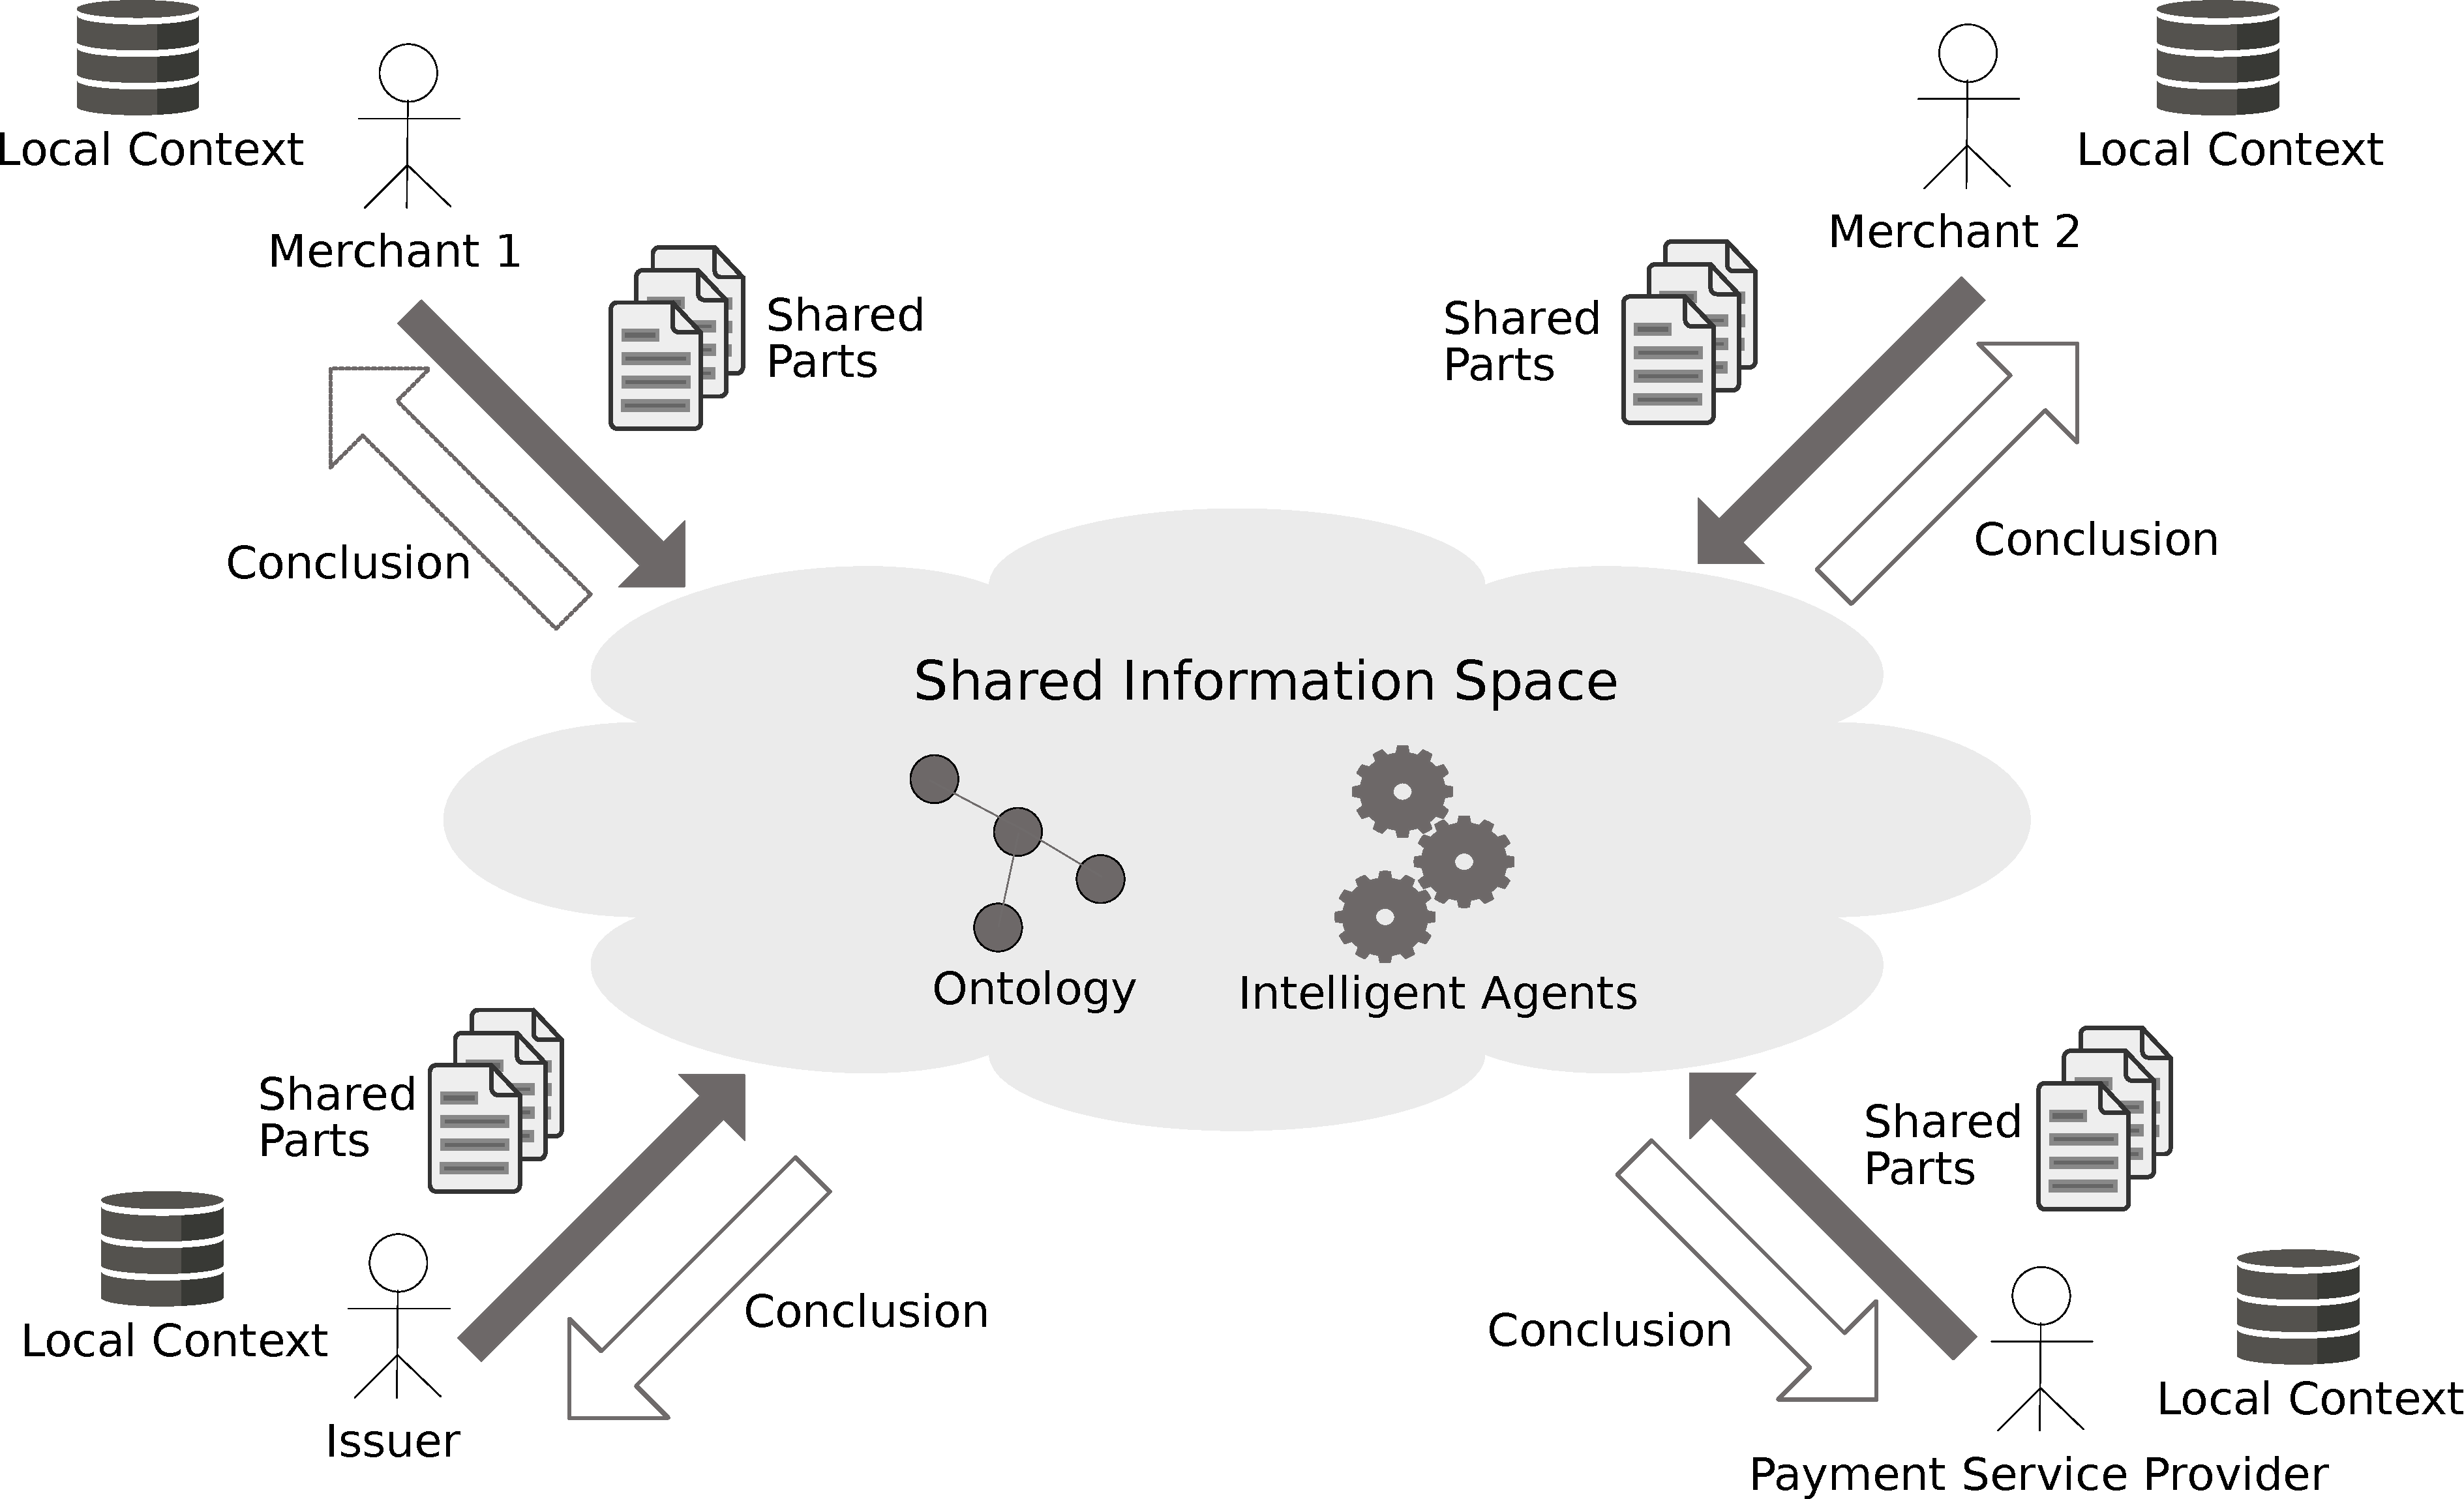
\includegraphics[width=0.9\columnwidth]{images/system_overview.pdf}
	\caption{System Overview}
\label{fig:images_system_overview}
\end{figure}

Due to the fact that data from various sources has to be combined into a shared understanding of the E-commerce activities of a consumer, there is the need to harmonize and transform the information into a shared data model. Based on the discussion in Chapter~\ref{cha:context_analysis} and the analysis of the information each stakeholder holds and transmits to others, the following initial schema can be conducted (see Figure~\ref{fig:images_data_model}). \\

\begin{figure}[!ht]
  \centering
  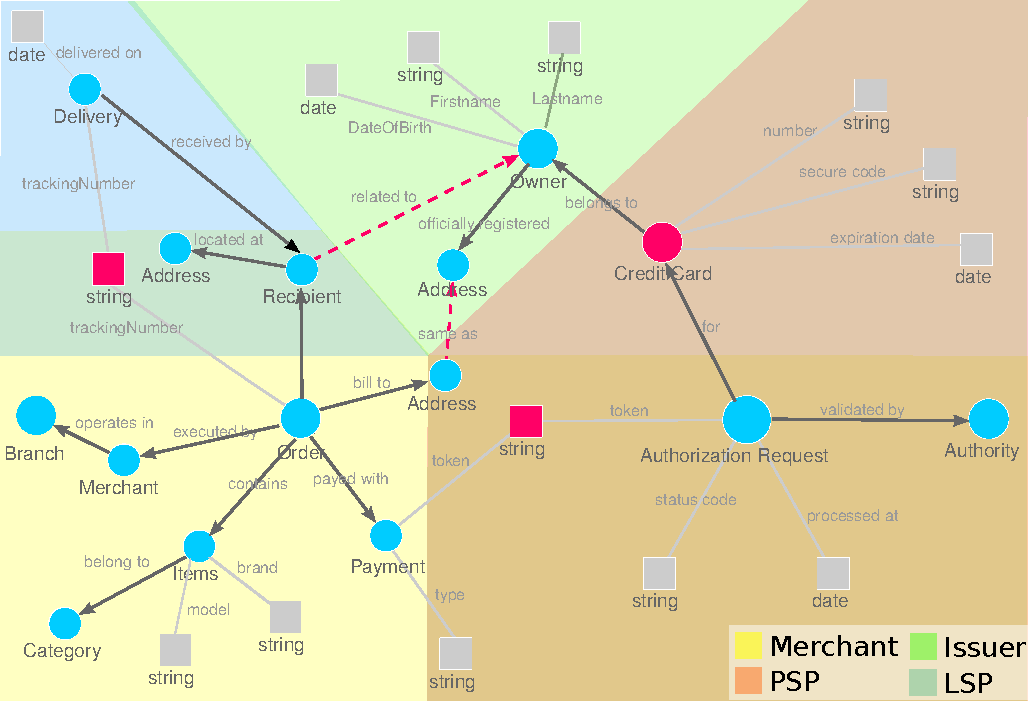
\includegraphics[width=0.9\columnwidth]{images/ontology_scenario_1.pdf}
  \caption{Information relations between stakeholders (green: Issuer, red: \gls{PSP}, yellow: Merchant, blue: \gls{LSP})}
\label{fig:images_data_model}
\end{figure}

As one can see there are connection points between stakeholders, that can be used as reference when trying to combine the information from each of them. These connection points are: \@

\begin{enumerate}
  \item \textbf{payment token}: shared between merchant and \gls{PSP}
  \item \textbf{tracking number}: shared between merchant and \gls{LSP}
  \item \textbf{credit card}: shared between issuer and \gls{PSP}
\end{enumerate}

In addition to the connection points one can also see the validation points in the visualization. These criterias are: \@

\begin{enumerate}
  \item \textbf{billing address}: the billing address of the order has to match the registered address of the owner of the credit card used
  \item \textbf{recipient}: the recipient of the delivery should be related to the owner of the credit card
\end{enumerate}

% section system_overview (end)
